
 \section{Heuristic feedback}  
In addition to monitored metrics which constitute the basic set of states, there are a set of states that can be deducted from monitored metrics using simply defined system blocks or transfer functions over time. In the following section we briefly  mention the most common examples of this kind that are commonly used in resource provisioning. Later we introduce examples that combine these patterns in order to form a closed control loop. 

The most common simply deductible state variable is \textit{counter} state variable is a numerical variable that maintains the algebraic sum of number of times an event occurs. The counter is usually implemented using a variable that is incremented, decremented based on some pre-conditions.
As a special case \textit{duration} state variable, measures the length of time some action or event has been occurring (e.g., system uptime)
We use  this duration state variable in the following manner. 
 We assume $t'^{ija}$ denotes the duration for which a given metric has been breaching a specified threshold (i.e., time spent in the violation zone).  It is maintained using the following transfer function: 
\[
  t'^{ij\mathtt{a}}_{k+1} = \left\{ 
  \begin{array}{l l}
    t'^{ij\mathtt{a}}_k+1 & \quad \text{if $\varrho^{ij}_k > \mathtt{a}$}\\
    0 & \quad \text{if $\varrho^{ij}_k < \mathtt{a}$}\\
  \end{array} \right.
\]

 We also introduce a \textit{step-like} state variable, which takes value of another state variable and maps it to a value from a finite set. 
In autoscaling this is used to construct a  vote $\psi^{ij\mathtt{a}\mathtt{e}}_k $ of acquiring and/or releasing a resource by a single server 
\[
\psi^{ij\mathtt{a}\mathtt{e}}_k = \left\{ 
 \begin{array}{l l}
    -1 & \quad \text{ if } t'^{ij\mathtt{a}}_k > \mathtt{e} \\
    1 & \quad \text{ if } t'^{ij\mathtt{a}}_k < \mathtt{e} \\
    0 & \quad \text{otherwise} \\
  \end{array} \right.
\]

 By combining the duration and step-like pattern, we construct an \textit{alert} state variables, which 
maps the duration of continuous occurrence of an event to discrete value ( here a vote). 
 
%An example of such an alert specification revolving around \texttt{cpu-idle} metric of a computer system is presented in Table \ref{tab:alerts-spec-example}.   
%\begin{scriptsize}
%\begin{table}[h]
%\center
%\begin{tabular}{ |l|l|l| }
%\hline 
%Condition & Duration & Action \\
%\hline \hline 
%If \texttt{cpu-0/cpu-idle} is $<$ \texttt{a\%} &  \texttt{x} minutes & vote to \texttt{grow} \\
%If \texttt{cpu-0/cpu-idle} is $>$ \texttt{b\%} &  \texttt{y} minutes & vote to \texttt{shrink} \\
%\hline 
%\end{tabular}
%	\caption{Template of alert specifications.}
%	\label{tab:alerts-spec-example}
%\end{table}
%\end{scriptsize}

In this example, adding multiple alerts defined based on multiple metrics is also possible . For example, for an application which is both memory and CPU intensive at times, one can set up alert specifications based on both CPU utilization and available memory. 
In such case 

a resource aggregate vote $\xi^{j}_k$ for each resource based on the aggregation of individual threshold votes
can be obtained using an \textit{aggregator} state variable as follows: 
\[
\xi^{j}_k=\sum_{i\mathtt{a}\mathtt{e}} \psi^{ij\mathtt{a}\mathtt{e}}_k
\]

to summarize, for a simple autoscaling scenario we took the following variables as the state vector (i.e., $x_k$): 
\[
 x_k=\left[
 \begin{array}{l l}
    t'^{ij\mathtt{a}}_{k} & \quad \forall i,j,\mathtt{a} \\
    \psi^{ij\mathtt{a}\mathtt{e}}_k  & \quad \forall i,j,\mathtt{a},\mathtt{e} \\
    \xi^{j}_k  & \quad \forall j
  \end{array} \right] 
\]
A more complete list of patterns used to define state variables is discussed in \ref{tab:alerts-state-variables}. 


%\begin{table*}[t]
%	\centering
%\begin{tabularx}{\linewidth}{ r X }
%%\begin{tabular*}{0.90\textwidth}{|l|l|}
%\hline \\
%Alert Target & Metrics \\
%\hline \\
%Counter  &
%Measures how many times an event or action has occurred using discrete, constant increments (e.g., number of active connections).\\
%Duration  &
%Measures the length of time some action or event has been occurring (e.g., system uptime)\\
%Average  &
%Measures the statistical average of some numerical or temporal parameter.\\
%Maximum  &
%Measures the statistical maximum of some numerical or temporal parameter.\\
%Minimum  &
%Measures the statistical minimum of some numerical or temporal parameter.\\
%\hline \\
%\end{tabularx}
%	\caption{List of the patterns for defining state variables.} 
%	\label{tab:alerts-state-variables}
%\end{table*}


%An architecture for a reactive autoscaler is presented in Figure \ref{fig:reactive-resource-provisioner}.
%
%++++++++
 
based on this state vector one can configure an autoscaler to launch an additional instance when a 
majority of the servers are being overworked. 
Once the number of targets voting to grow exceeds a specified \textit{decision threshold} (e.g. 51\%) a scaling action will be performed. 
Likewise, the policy function should remove an instance when servers are under-utilized due to a decline in traffic.
% If, after resizing, the number of instances falls within the interval defined between \textit{min\_instances} and \textit{max\_instances} 
a scaling action will launch/terminate a number of instances configured by a \textit{resize number}. 
In this case the policy $\mu(x_k)$ defined to derive resource reservation for next step from constructed state was based on the value of the resource votes as follows: 
\[
  \kappa_{k+1} = \left\{ 
  \begin{array}{l l}
    \text{acquire} & \quad \text{if $\left(\sum_{j=1..N} \xi^{j}_k\right)/N > \mathtt{d}$}\\
    \text{release} & \quad \text{if $\left(\sum_{j=1..N} \xi^{j}_k\right)/N < \mathtt{d}$}\\
    \text{none} & \quad \text{otherwise} 
  \end{array} \right. 
\]

% modify the above thing to take into account these stud 
To avoid trashing once a scaling action occurs, the system should not be allowed to perform another scaling action until a \textit{refractory period} has passed. This is because, it takes some time to launch a new server (i.e. copying the server image to a physical host and booting a VM from it) 
before it becomes operational and starts offloading some of the work from the overworked instances.
This is implemented by having an \textit{duration} state variable $t_k$ on the duration past from an autoscaling action \footnote{This type of state formation is denoted in figure ... by an arrow that takes 'the actions' from 'policy function' block and feeding it back to the  'state formation' block. }:    
\[
  t_{k+1} = \left\{ 
  \begin{array}{l l}
    t_k+1 & \quad \text{if $\kappa_{k}=$ 'acquire' or 'release' }\\
    0 & \quad \text{if $\kappa_{k}=$ 'none' }\\
  \end{array} \right.
\]

and modifying policy function as: 
\[
  \kappa_{k+1} = \left\{ 
  \begin{array}{l l}
    \text{acquire} & \quad \text{if } \left(\sum_{j=1..N} \xi^{j}_k\right)/N > \mathtt{d}  \wedge \neg( t_k < \mathtt{e} )\\
    \text{release} & \quad \text{if } \left(\sum_{j=1..N} \xi^{j}_k\right)/N < \mathtt{d} \wedge \neg( t_k < \mathtt{e} ) \\
    \text{none} & \quad \text{otherwise} 
  \end{array} \right. 
\]

After an autiscaling action, if additional servers make enough impact, the triggered alerts in some targets disappear, the number of votes decreases below the decision threshold and autoscaling will be stopped. Otherwise, after the refractory period, a new autoscaling action will be triggered again. 


% As an example of a common scenario is when the maximum and toggle patterns for a control loop. In this case the toggle condition, instead of a Boolean parameter, is obtained by comparing a variable to a maximum parameter. 
% For example, a web server might increase the connection poll size if the maximum number of faults per second exceeds some amount:
%\begin{lstlisting}[label=some-code,caption=Some Code]
%update(maxReqPerSec);
%boolean increaseSize=curFaultRate> maxFaultRate;
%if (increaseSize){
%    maxFaultRate= curFaultRate + 
%(curFaultRate -maxFaultRate)*0.1
%	conPoll.setSize(curSize*1.2);
%}
%�
%\end{lstlisting}
%
%In this example, the reflexive parameter (e.g. maximum number of faults per second) is used to control the execution of some behavior (i.e. increasing the size of connection-poll).
%

%\begin{table*}[t]
%	\centering
%\begin{tabularx}{\linewidth}{ r X }
%%\begin{tabular*}{0.90\textwidth}{|l|l|}
%\hline \\
%Alert Target & Metrics \\
%\hline \\
%Enumerable &
%Controls the behavior of the system through some finite set of states (e.g., thread priorities, algorithm selection).\\
%Toggle  &
%Enables or disables a behavior of the system (e.g., caching allowed).\\
%Capacity  &
%Limits how large (i.e., memory footprint) a resource can grow (e.g., buffer limits).\\
%Threshold &
%Limits the number of times an event or action can occur (e.g., prevent new connections).\\
%Period  &
%Controls the frequency with which an action or event is triggered (e.g., garbage collection).\\
%Timeout  &
%Limits the length of time an action has to complete before it will be interrupted (e.g., reading bytes from a network connection).\\
%\hline \\
%\end{tabularx}
%	\caption{List of the metrics used in defining autoscaling alerts.}
%	\label{tab:alerts-metrics}
%\end{table*}
%+++++++
%A behavioral pattern: Toggle
%
%As mentioned earlier a toggle pattern is characterized by presence of a variable (usually Boolean) which controls if a part of the program is executed or not (i.e. enabled or disabled). 
%
%Toggle pattern is usually manifested in the source code as an if-statement which changes the control sequence based on evaluated value of a toggle field.
%A temporal pattern: Delay
%
%A delay prevents a behavior from occurring for some specified length of time. 


%As it turns out, a solution to a feedback problem is provided by optimal control which avoids these issues. Such a solution is described in detail in the following section.

% 
% 
% ++++++
% For a autoscaler, the state is composed of state of (i) the cloud with respect to the customer including state of \textit{reservation contracts}, resource availability, and resource price and (ii) the state of software system (denoted by $x''$). From now on we refer to state variables regarding cloud as \textit{Cloud state}. 
% 
% +++++++++++++++++++
% In case of autoscalers, the choice of system attributes that constitute a system state is up to the designer of the autoscaler. State attributes can be observed, estimated, part of cost function or not. One important decision is to include what portion of attributes $y_k$ involved in cost function.  The principle is to capture enough information in state to derive efficient decisions. % In section ?ref we further explore different choices of state. %use a technique to figure out proper 


%Another form of scaling can be substituting an instance with more powerful one (i.e. more cores and memory). The former type of scaling is called horizontal scaling while the later is called vertical scaling. One must notice that, only a clustered service can be configured for horizontal autoscaling. For example, some monotonic databases might not be cluster-able, that is even if replicated, they cant provide the originally provided consistency level by a single server. For this reason, the best candidates for horizontal scale-ups in transactional e-commerce applications, are frontends (who are serving static content) and application servers (which are serving dynamic content).


\begin{figure}[htb]
	\centering
	% 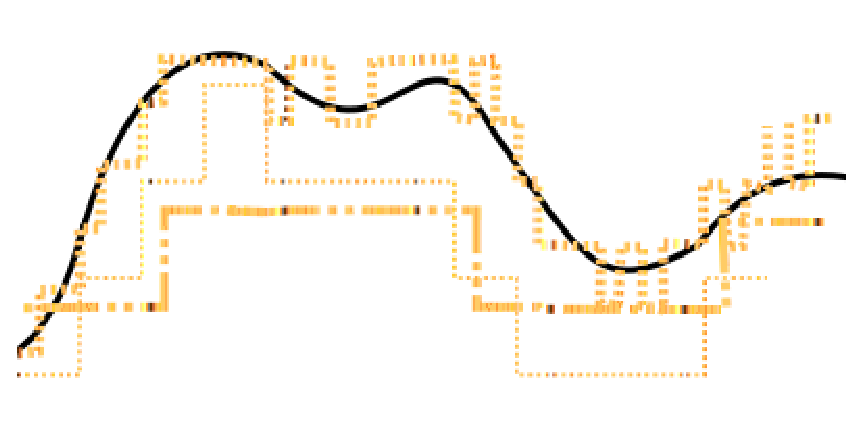
\includegraphics[width=0.45\textwidth]{./image/pre/workload6.eps}
	% workload6.eps: 0x0 pixel, 300dpi, 0.00x0.00 cm, bb=14 14 413 207
	\caption{Effect of different autoscaler configurations on the scaling behavior.}  
	\label{fig:different-autoscaler-configuration}
\end{figure}
Figure~\ref{fig:different-autoscaler-configuration} schematically represents the behavior of three different autoscaler configurations on the scaling behavior. The workload is represented by a solid line, while the number of instances (an a representative of autoscaler behavior) in three different configurations is represented by step-like functions. 


% \cite{rightscale_autoscaling}.
% and assessed the capabilities of the approach and compared it to our past experiences using control theoretic approach. 

%%All platform instances were built atop VM instances running Ubuntu 9.10 i386 or CentOS 5.4 i386  (i.e., front end servers, application server instances, and databases) and configured as {\it m1.small} instances (i.e., 1.7 GB memory, 1 EC2 Compute Unit, 160 GB instance storage, 32-bit platform and moderate I/O Performance).
%In a real experiment, we deployed a simple web application as a multi-tiered topology consisting of two front-end servers running Apache, HAProxy and Tomcat, a backend database running MySQL 5.0 and a server array of Tomcat instances.
%We used Amazon Web Services (AWS) as the IaaS provider. 

Three different elasticity policies were designed to drive the autoscaling actions of the application server tier. 
These rule sets utilized different settings of the configurable parameters mentioned above and are presented in Table~\ref{tab:ps}.  
%The FIFA '98 workload~\cite{arlitt_workload_2000} was used as a representative workload against which the application was run.

\begin{table}[h]
\center
\begin{tabular}{ ||c || c | c | c| }
  \hline
   Parameter & $EP_1$ & $EP_2$ & $EP_3$ \\
   \hline \hline                       
   \texttt{resize numbers}      & 1 & 1 & 2  \\
   \texttt{decision threshold}	& 51\% & 51\% & 51\% \\
   \texttt{operating interval}	& [50,45] & [55,40] & [55,50] \\
   \texttt{decision duration} 	& 7 min & 7 min & 8 min \\ 	
   \texttt{refractory\_period} 	& 8 min & 8 min & 6 min \\
   \texttt{instance bounds}	& [2,20] & [2,20] & [2,20] \\
  \hline  \hline
\end{tabular}
\caption{Parameter settings defining the three elasticity policies (EP).}\label{tab:ps}
\end{table}
 
 A plot of the platform instances purchased over time and the average utilization of a server in the cluster is presented in Figure~\ref{fig:workload-versus-num-servers}\subref{fig:sub2} and \subref{fig:sub3} for each set of rules. 
It is noticeable that different rule sets result in different elastic behavior for the same workload.  


%\begin{figure}[h]
%	\centering
%	\subfloat[][]{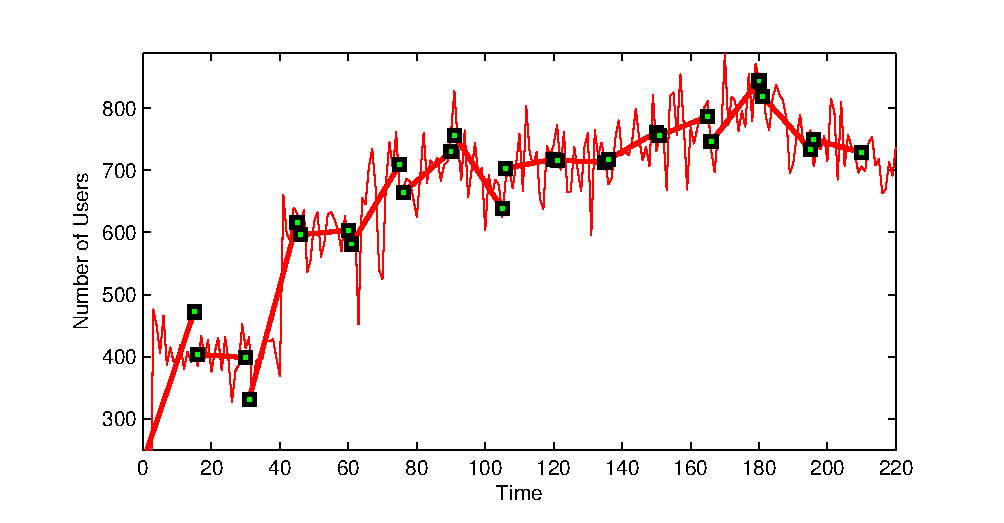
\includegraphics[width=0.50\textwidth]{image/result3/rbe-regression-num_users2.eps}\label{fig:sub1}} \\
%	\subfloat[][]{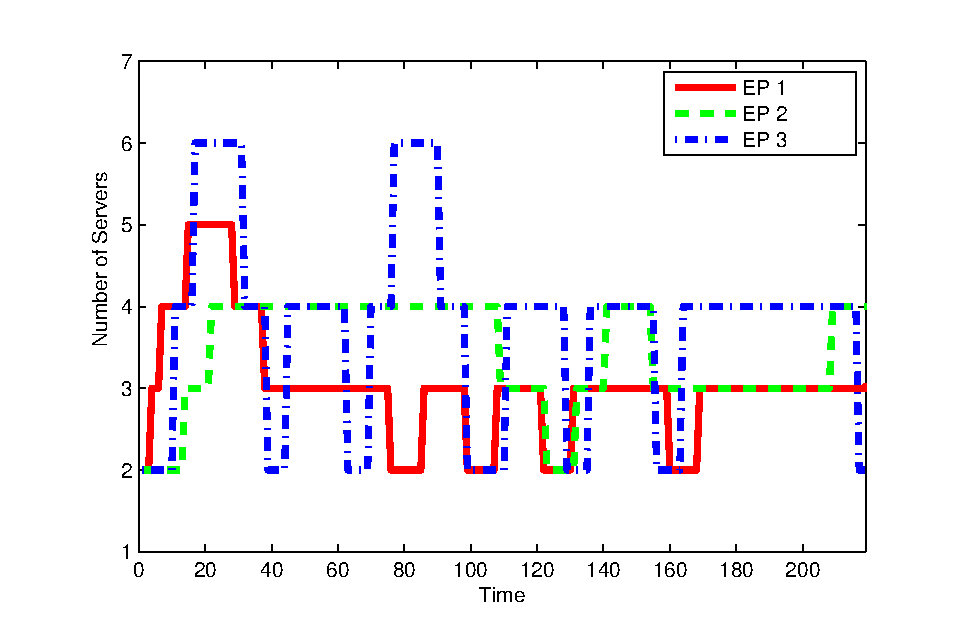
\includegraphics[width=0.50\textwidth]{image/result3/manager-servers2.eps}\label{fig:sub2}} \\
%	\subfloat[][]{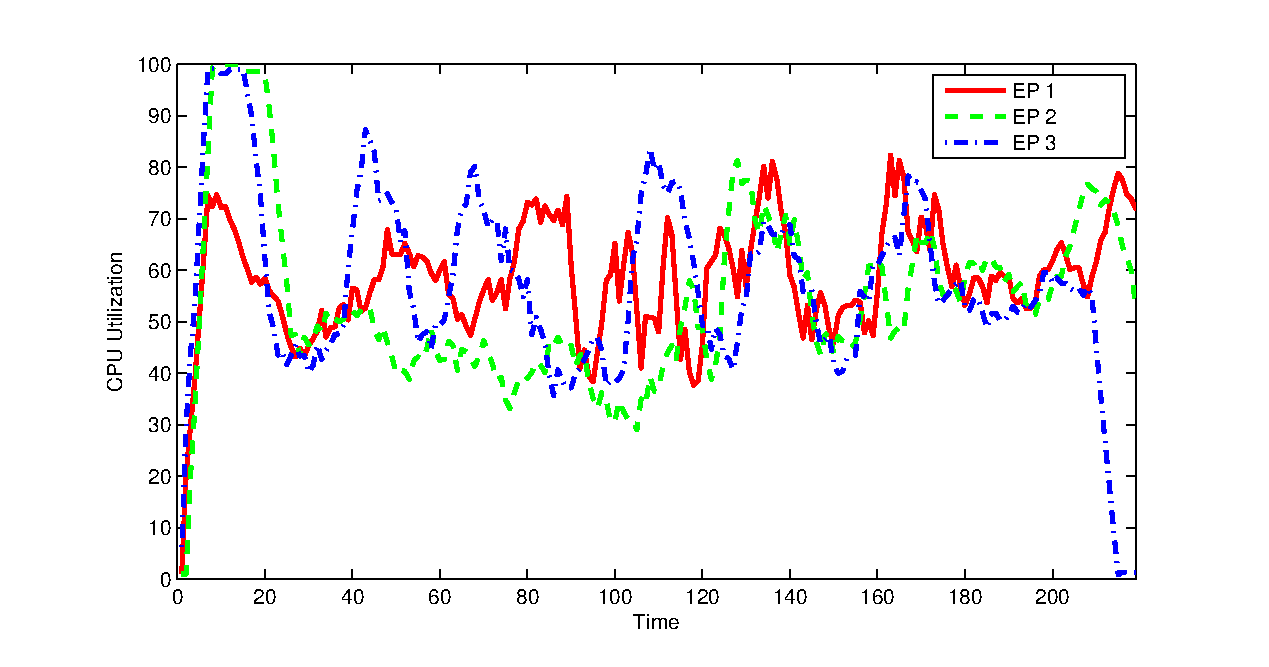
\includegraphics[width=0.50\textwidth]{image/result3/cpu-utilization.eps}\label{fig:sub3}}
%	\caption{The \subref{fig:sub1} workload  versus \subref{fig:sub2} the number of fired servers and \subref{fig:sub3} the average utilization of a server in the cluster for three elasticity policies ($EP_1$, $EP_2$ and $EP_3$) .}
%	\label{fig:workload-versus-num-servers}
%\end{figure}

% \begin{figure}[h]
%   \centering
%     \includegraphics[scale=.35]{imgs/graph1.pdf}
%   
% \caption{A plot of the number of additional platform instances acquired and
% released elastically  versus time for each policy set ($P_1,P_2$ and
% $P_3$).}\label{fig:graph1}
% \end{figure}

The figure shows the ability of the the constructed control loop constrain a certain metric in an operating region. 
However there were definite problems with this type of control loop:
(i) the proper number of alerts, and the associated values for \texttt{a},\texttt{e},\texttt{d} could not be deduced automatically, in a way that satisfies performance metrics requirements. 
%There are various ways that one can configure an autoscaler. 
For example, for a transactional application deployment with $l$ hosts, $m$ available metrics, and $n$ predicates for defining conditions,
 each host might choose a subset of $[\text{predicates} \times \text{metrics}]$ (i.e. $2^{n*m}$ choices) to define its alerts.
These alternatives, together with global configuration parameters \textit{decision threshold}, \textit{resize number}, \textit{min\_instances}, and \textit{max\_instances} form a huge configuration space and this makes it hard to investigate each configuration parameter's impact on the behavior of the autoscaler.    
(ii) It is not clear how to manage the resource cost by tuning the policy or state definitions. 

The solutions to these two problems are introduced in the next chapters. 
However, here we only try to give a rough explanation of how configuration parameters will affect the (i) acquired resources (ii) performance metrics.  
% With several tests we concluded a simple scheme for describing the effect each parameter, however. 
% 
% just added before final 

%One way of characterizing an autoscaler's behavior is to show how it reacts to the perturbations in the environment (i.e., disturbance input to the system). 
%Rather than accessing the effectiveness of an autoscaler in achieving objectives defined on system output(s) this characterization helps in comprehending autoscaler behavior in general. 
%One can aim at building mathematical model for behavior of the autoscaler.
%For example by considering autoscaler decision (i.e. here number of instances) over time as a transfer function $F(z)$ over configuration parameters (i.e. subset of predicates applicable to system outputs) and system output (e.g. average server utilization): 
%\[\text{servers}(z) = F_\text{configuration}(z) \text{sys-out-metric}(z)\] 
%servers = f(configuration,utilization)
% knowing that autoscaler decision together with workload component make inputs of the system $G(z)$: 
%\[\text{sys-out-metric}(z) = G(z)[\text{servers}(z)+\text{workload}(z)]\] 
%utilization = g(servers,workload)
%one might be able to construct a transfer function $H(z)$ from workload component to the autoscaler decision (for a specific system)
%\[\text{servers}(z)=H_\text{configuration}(z)\text{workload}(z)\]
%servers=f(configuration,g(servers,workload))
%The approach we took in this work was to roughly characterize autoscaler based on its decisions (over configuration space) rather than modeling it formally. 
% roughly derive properties of
% We considered autoscaler as a transfer function which takes the workload function and maps it to a function representing number of active instances over time (lets call it \textit{node curve}). 
 % We consider the autoscaler as a transfer function which takes the workload and maps it to a function representing the number of active instances over time (i.e., a {\it node curve}).   
% Next, 
% We qualitatively categorized the effect of each configuration parameter on the behaviour of autoscaler.  %this transfer function.
%To further simplify it, we assumed there is only one subsystem under autoscaling (e.g. application server tier) with homogeneous instance types 
%and CPU utilization is the only metric used in defining alert types.
%
%In our experiments all the alerts in all targets were identical and based on the template introduced in Table \ref{tab:alerts-spec-example} (e.g., two alerts where defined, one for scale-up action is case of over-utilization and one for scale-down in case of under-utilization).
%Over-utilization is considered when CPU idle time is less than the lower bound \textit{cpu-idle-lb} and underutilization is defined as when CPU idle time is more than the upper bound \textit{cpu-idle-ub}.
%The interval $[\text{\textit{cpu-idle-lb}},\text{\textit{cpu-idle-ub}}]$ formed by these two bounds, together with {\it decision threshold}, {\it refractory period}, {\it decision durations}, {\it resize numbers}, and $[\text{{\it min\_instances}},\text{{\it max\_instances}}]$ interval form a simpler configuration space that we investigate in this work. 
%We summarize the effect of different autoscaler configurations on the scaling behavior as follows:

%%\begin{description}
%\textbf{Operating interval} formed by $[\text{\textit{cpu-idle-ub}},\text{\textit{cpu-idle-ub}}]$ is the main tool in configuring the long term size of the cluster. 
%It basically forces the autoscaler to act until the cluster reaches the desired average operating interval (here in terms of CPU idle time, e.g. $[20\%,30\%]$ idle).
%
%If the desired operating interval is located at high CPU idle values (e.g. $[40\%,50\%]$), there will be a lot of instances launched.
%Autoscaling will eventually stop due to the increase in the number of idle instances, resulting in less alerts being signaled (as the triggering threshold is no longer reached). 
%Notice that the autoscaling action is only performed if the intensity of the workload can get cluster nodes to the desired operating point. Thus, if 
%the operating point is configured when nodes are fully utilized (e.g. $[0\%,10\%]$ CPU idle time), the cluster might become unresponsive for low intensity workloads.
%
%If this interval is configured to be narrow and it is placed in an operating area reachable by the workload, it will make the autoscaler sensitive to changes. Such an autoscaler  would do some thrashing just to keep the operating point at this narrow interval. If the interval is wide, the cluster will be less responsive, and the cluster utilization will have more space for variations. 
%
%\textbf{Decision duration} contributes to the responsiveness of the cluster. A shorter decision duration for each node results in a quicker response and, thus, it is better at detecting highly variable workloads (e.g. a workload that changes direction every 15 minutes). 
% In case of steady or monotonically increasing/decreasing workloads the cluster is going to stabilize on a specific size no matter what decision duration is. 
%% Note that, assigning a value lower than server launch time would result in catastrofy in some cases because the lanched servers might be heavily utilized after booting and thus make the cluster oversize constantly grow by voting to grow.
%
%\textbf{Resize numbers} represents the amount of servers to add or remove should a decision threshold (i.e., quorum) be reached  (e.g., 51\%). 
%This has a short term effect on the size of the cluster by making it grow or shrink faster. This might be useful for heavily increasing or decreasing workloads. However, in a long run for a lightly changing workload this might only have effect on smoothness of cluster size over time. 
%
%\textbf{Decision threshold} is global parameter closely related to decision duration, which can affect the responsiveness of the cluster specially in a heterogeneous clusters.
%In a heterogeneous cluster, nodes with less processing power might reach the saturation level faster. In this case a lower decision threshold might result in a better autoscaling decision. The same applied to cluster composed of two different types of nodes (e.g. frontend and application server) where the load on one type of node is higher than the other (e.g. a web application with lots of demand on static resources would result into more utilization at the frontend). 
%
%\textbf{Instance bounds} formed by $[\text{{\it min\_instances}},\text{{\it max\_instances}}]$ acts as constraint on the size of the cluster. 
%
%\textbf{Refractory period} is the interval of time which follows an autoscaling action during which no autoscaling actions may occur.  
%% can determine how well the cluster can resize for a changing workload. 
%With small refractory periods, the cluster makes resizing decisions more frequently resulting in more responsive behavior. 
%% \end{description}
%
%% Votes are aggregated at the Server level, so if a Server has multiple alerts that are using the same Voting Tag (e.g. MyArray), the Server will only have a single aggregated vote. 
%%  For example, you might have an application that's both memory and cpu intensive, so you create an alert specification that scales based on 'memory' and another alert specification that scales based on 'cpu'.   In such cases, there could be a situation where both alerts are triggered on a single Server.  Perhaps the 'memory' alert triggers a scale up (grow) action while the 'cpu' alert triggers a scale down (shrink) action.  In such cases, the votes would cancel each other out and a Server's Voting Tag would be set to 'none' and no vote would be made for either scaling action. (1grow - 1shrink = none)  
%% 
%%   So if there are 5 Servers voting to grow based on a triggered 'cpu' alert and another 5 Servers that are voting to grow based on a triggered 'memory' alert, the total number of votes to grow the array is 10.  
%
%%++++++++++
%% Policy.new({:increment=>1}),
%%            Policy.new({:decrement=>1}),
%%            Policy.new({:rest=>8}),
%%            Policy.new({:decision_thresh=>51}),
%%          # 100% means idle
%%          # 40% means relatively busy
%%            Policy.new({:cpu_idle_value=>45, :operator=>"lt",:vote_increase_duration=>7}),
%%          # 60% means relatively idle
%%            Policy.new({:cpu_idle_value=>50, :operator=>"gt",:vote_decrease_duration=>7}),
%%            Policy.new({:min_count=>0}),
%%            Policy.new({:max_count=>10})
%
%% ++++++++++
%%  subsection{Autoscaling for Grids} 
